% begin_generated_IBM_copyright_prolog                             %
%                                                                  %
% This is an automatically generated copyright prolog.             %
% After initializing,  DO NOT MODIFY OR MOVE                       %
% ================================================================ %
%                                                                  %
% (C) Copyright IBM Corp.  2011, 2011                              %
% Eclipse Public License (EPL)                                     %
%                                                                  %
% ================================================================ %
%                                                                  %
% end_generated_IBM_copyright_prolog                               %
\section{History of Blue Gene Workloads}

\subsection{First Generation Blue Gene (BG/L aka Blue Gene ``Light'')}
\label{sec:BGL}

Highlights/Features:
\begin{itemize}
\item Initial release supports HPC Message Passing Interface (MPI) workloads and jobs occupy multiples of 512 compute nodes.
\item Second release supports running HPC jobs on as few as 32 compute nodes.
\item Third release adds limited support for HTC single-node jobs.
\end{itemize}

The term ``light'' indicated that this was the first, smallest, and therefore ``light'' version of a
new supercomputer architecture that would grow into larger and more powerful designs in the future.
The stated goal of BG/L was to enable massively parallel applications to run at unprecedented
scales. The flagship BG/L machine, developed in a partnership between IBM and Lawrence Livermore
National Laboratory (LLNL), consisted of 64 racks of compute hardware, comprising 65,536 compute
nodes, and 131,072 processor cores. This machine achieved the top spot on the Top500 list of
supercomputers in November of 2004 \cite{website:top500November2004}, and held that position for an
unprecedented seven consecutive lists after being expanded to 104 racks. The machine was built for
scaling large applications, with relatively little emphasis placed on running many small jobs. In
Blue Gene, the term ``block'' is used to describe how the machine hardware is partitioned into
groups of compute nodes or I/O nodes. Collections of I/O nodes on BG/Q are referred to as ``I/O
blocks'' and collections of compute nodes are referred to as ``compute blocks''. In BG/L and BG/P
systems, only compute blocks existed and were simply called blocks. In
the initial design of the machine, the smallest block of the machine that could be used to run a job
was 512 compute nodes, or a half rack. Furthermore, a job had to occupy the entire block. This was
not considered to be a significant limitation, since the machine was designed with a priority of
running large jobs, and with a 64 rack machine one could run as many as 128 simultaneous jobs.
However, many customers expressed an interest in smaller machines, and some required only a single
rack system. It became clear that the smaller machines would require the ability to subdivide the
system in units with less than 512 compute nodes.  Software features were added to enable blocks
containing as few as 32 compute nodes. This was a significant enhancement to the usability of the
machine. The Blue Gene architecture suddenly became relevant to customers that would conceivably
never run a job that occupied the entire machine, and had workloads that did not scale to thousands
of parallel tasks. Now they could subdivide the machine into many smaller blocks, and run many
simultaneous jobs, and still get the benefits of a Blue Gene, such as the compute density of 1,024
compute nodes in a single rack, and the unparalleled power efficiency.

Even with the features added to enable smaller blocks, each job still had to be a parallel,
multi-node job. MPI based programs had to be equipped to break a problem down into multiple, smaller
pieces of work. This was always the stated purpose of the Blue Gene architecture, and yet there was
customer interest in expanding its use to other workloads, and not all of those workloads used MPI.

Also, there was still a requirement that each block had to contain at least one I/O node connected
to the functional network to enable I/O. This was a hardware limitation due to the collective network
used by the compute nodes to communicate with the I/O node. This meant that in order to create the smallest blocks of
32 compute nodes, a rack of 1,024 compute nodes had to be equipped with 32 I/O nodes. This was not a
common machine configuration for BG/L, since most customers chose a ratio of only 8 or 16 I/O nodes
per rack, due to hardware costs and Ethernet switch capacity. As a result, even though 32 node
blocks were enabled by the software, there were not many installed racks of BG/L that had the
hardware configured to take advantage of this feature.

So there remained a need to enable more simultaneous jobs on BG/L, and to somehow circumvent the
hardware limitations that required an I/O node per job. With these goals in mind, further work was
done on BG/L to enable rudimentary support for HTC style applications  \cite{marshall:09}. The
strength of BG/L was in its robust performance of parallel applications, and it was best known as an
extreme scaling HPC machine. However, some customers started to consider the possibility of using
BG/L as a cluster of many small nodes, each running independent tasks. This was very different than
anything that had been done on a BG/L machine, and not something that the Control System software
was equipped to handle. As a proof-of-concept, a group of software engineers created an HTC model
that could be achieved by executing a \emph{launcher} program on all of the compute nodes of a BG/L
block. From the perspective of the Control System, this was a single binary executable started on
all of the compute nodes in a block, so at that level, it was no different than a typical HPC
application. But this \emph{launcher} program was really just a basic mechanism to execute different
applications on different compute nodes using special support in the CNK \cite{peters:08}. While
this model demonstrated a method of running many different executables on a single BG/L block, it
had several key limitations that made its widespread adoption impractical. One drawback was that the
Control System was unaware of the different applications running and had no way to do tracking and
accounting of the individual jobs. Because of the \emph{launcher} based design, jobs could not be
signaled or killed and it was impossible to separate any job output written to standard output.
Also, all of the launched jobs were run under the same user which was a security limitation.

This initial proof-of-concept showed that it was possible for Blue Gene to handle both ends of the spectrum. The worlds largest parallel jobs as well as the smallest single-node jobs could be supported by the Blue Gene architecture. It also became apparent that tighter integration with the Control System and kernel layer would be necessary for HTC workloads to be widely accepted on Blue Gene.

\subsection{Second Generation Blue Gene (BG/P aka Blue Gene ``Petaflop'')}
\label{sec:BGP}

Highlights/Features:
\begin{itemize}
\item Stronger integration for HTC workloads in Control System and kernel layer.
\item Lightweight HTC job submission design along with a multiplexer to handle thousands of job proxy client connections.
\end{itemize}

BG/P was designed as a petaflop capable machine and the flagship 72 rack system has a theoretical peak
performance of one petaflop \cite{website:jugene}. There were many new features and enhancements made in BG/P.
One of the key new software elements was an HTC job submission mode that was fully integrated into the Control
System software. Figure \ref{fig:htcjobsubmission} shows the architecture and various components. This meant
that unlike the BG/L \emph{launcher} design, the BG/P design could allow users to submit single task jobs to
nodes within a block. Because the Control System was fully aware of every HTC job being run, each job could be
tracked and accounted for in the job history, output from jobs were not intermingled, and each job had a
distinct user associated with it. Several novel software ideas emerged from this HTC project due to the need
for fast and efficient job launch time. When running thousands of HTC style jobs, this setup time was a
critical factor and often dominated the total perceived execution time of the job itself. Due to this, much
focus was placed on providing a fast, lightweight, and efficient job submission path. The addition of a
multiplexer component on the job submission nodes, as well as I/O nodes, reduced the authentication overhead
and offloaded several verification tasks from the central daemon. Using prepared SQL statements to insert,
update, and remove entries from the database proved much more efficient than using dynamic queries.

\begin{figure}[!b]
    \centering
    \caption{BG/P HTC Job submission architecture.}
    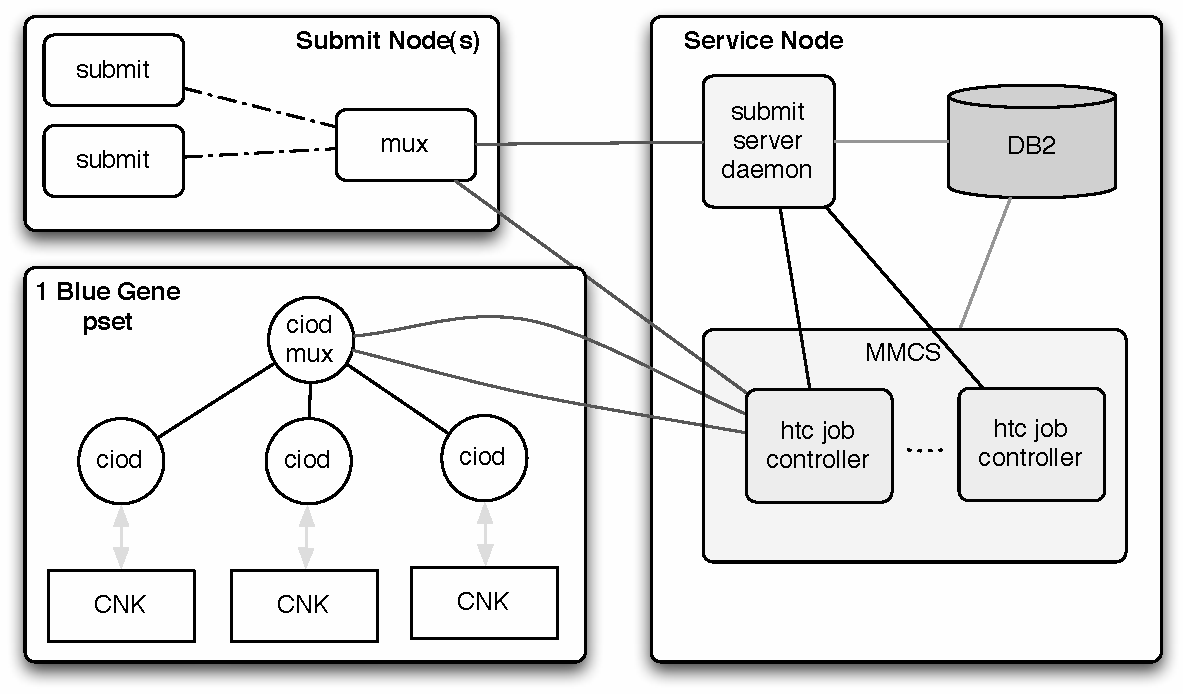
\includegraphics[width=3.5in]{bgp_htc_architecture}
    \label{fig:htcjobsubmission}
\end{figure}

Rather than being a proof-of-concept project like the BG/L version of HTC, the BG/P HTC software was
production level. This made a BG/P machine much more flexible in terms of the workloads that it could support.
A machine could be used for part of the day running massively parallel HPC applications, then spend another
part of the day processing thousands of independent tasks for an HTC workload. Even a blend of HTC and HPC
applications could be running simultaneously on different blocks of the system.

The HTC features of BG/P have been used by many customers, and have indeed expanded the scope of possible
workloads that can run on Blue Gene. However, the work in this HTC space still left room for improvement. The
BG/P system software was restricted in an artificial way because a block could handle either single node HTC jobs or
HPC (MPI) type jobs but not a blend of the two. In order to switch between workload styles a block required
rebooting which was inefficient. For complete flexibility the ideal solution would be for a block to handle
all types of workloads without a reboot. Another area of concern was the multiple conflicting methods of job
submission. For HPC style jobs the \emph{mpirun} command was invoked, for HTC type jobs the \emph{submit}
command was used. The grand unification of multiple commands into a single comprehensive job submission
command would have to wait though until BG/Q when the Control System software could be restructured. 
